\chapter{Exercise 01}
\extitle{ImageProcessor}
\turnindir{ex01}
\exnumber{01}
\exfiles{ImageProcessor.py}
\exforbidden{None}
\makeheaderfilesforbidden


% ================================= %
\section*{Objective}
% --------------------------------- %
Basic manipulation of images via the Matplotlib library.


% ================================= %
\section*{Instructions}
% --------------------------------- %
Build a tool that will be helpful to load and display images in the upcoming exercises.\\
\\
Write a class named \texttt{ImageProcessor} that implements the following methods:
\begin{itemize}
  \item \texttt{load(path)}: opens the PNG file specified by the \texttt{path} argument and returns an array with the RGB values of the pixels in the image. It must display a message specifying the dimensions of the image (e.g. 340 x 500).

  \item \texttt{display(array)}: takes a numpy array as an argument and displays the corresponding RGB image.
\end{itemize}
You must handle these errors: if the file passed as argument does not exist or if it can't be read as an image, with an appropriate message of your choice.

\hint{You can use the library of your choice for this exercise, but converting the image to a numpy array is mandatory.
The goal of this exercise is to dispense with the technicality of loading and displaying images,
so that you can focus on array manipulations in the upcoming exercises.
}

% ================================= %
\section*{Examples}
% --------------------------------- %
\begin{minted}[bgcolor=darcula-back,formatcom=\color{lightgrey},fontsize=\scriptsize]{python}
from ImageProcessor import ImageProcessor
imp = ImageProcessor()
arr = imp.load("non_existing_file.png")
# Output :
Exception: FileNotFoundError -- strerror: No such file or directory

print(arr)
# Output :
None

arr = imp.load("empty_file.png")
# Output :
Exception: OSError -- strerror: None

print(arr)
# Output :
None

arr = imp.load("../resources/42AI.png")
# Output :
Loading image of dimensions 200 x 200

arr
# Output :
array([[[0.03529412, 0.12156863, 0.3137255 ],
        [0.03921569, 0.1254902 , 0.31764707],
        [0.04313726, 0.12941177, 0.3254902 ],
        ...,
        [0.02745098, 0.07450981, 0.22745098],
        [0.02745098, 0.07450981, 0.22745098],
        [0.02352941, 0.07058824, 0.22352941]],

       [[0.03921569, 0.11764706, 0.30588236],
        [0.03529412, 0.11764706, 0.30980393],
        [0.03921569, 0.12156863, 0.30980393],
        ...,
        [0.02352941, 0.07450981, 0.22745098],
        [0.02352941, 0.07450981, 0.22745098],
        [0.02352941, 0.07450981, 0.22745098]],

       [[0.03137255, 0.10980392, 0.2901961 ],
        [0.03137255, 0.11372549, 0.29803923],
        [0.03529412, 0.11764706, 0.30588236],
        ...,
        [0.02745098, 0.07450981, 0.23137255],
        [0.02352941, 0.07450981, 0.22745098],
        [0.02352941, 0.07450981, 0.22745098]],

       ...,

       [[0.03137255, 0.07450981, 0.21960784],
        [0.03137255, 0.07058824, 0.21568628],
        [0.03137255, 0.07058824, 0.21960784],
        ...,
        [0.03921569, 0.10980392, 0.2784314 ],
        [0.03921569, 0.10980392, 0.27450982],
        [0.03921569, 0.10980392, 0.27450982]],

       [[0.03137255, 0.07058824, 0.21960784],
        [0.03137255, 0.07058824, 0.21568628],
        [0.03137255, 0.07058824, 0.21568628],
        ...,
        [0.03921569, 0.10588235, 0.27058825],
        [0.03921569, 0.10588235, 0.27058825],
        [0.03921569, 0.10588235, 0.27058825]],

       [[0.03137255, 0.07058824, 0.21960784],
        [0.03137255, 0.07058824, 0.21176471],
        [0.03137255, 0.07058824, 0.21568628],
        ...,
        [0.03921569, 0.10588235, 0.26666668],
        [0.03921569, 0.10588235, 0.26666668],
        [0.03921569, 0.10588235, 0.26666668]]], dtype=float32)
imp.display(arr)
\end{minted}
\begin{figure}[h!]
  \centering
  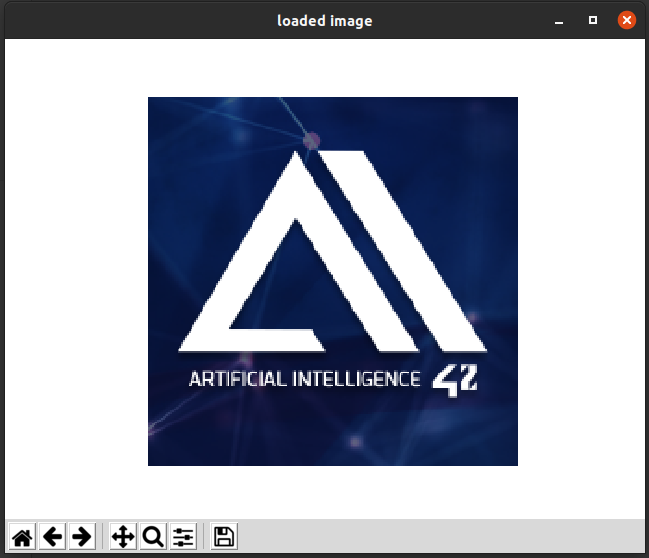
\includegraphics[scale=0.5]{assets/capture_display_img.png}
\end{figure}

The image must be displayed in a separate window when running in the console.